Per stampare un progetto oppure per esportare il progetto in formato PDF\ped{G} un utente deve essere iscritto ed autenticato. Per accedere alla pagina di stampa ed esportazione di un progetto l'utente deve premere il pulsante azzurro \textbf{My Project} posto in alto a destra sullo schermo. Una volta premuto si caricherà la pagina corrispondente. A questo punto l'utente deve selezionare il progetto da stampare o esportare dalla lista dei progetti in alto a sinistra.
Una volta selezionato il progetto apparirà al centro dello schermo il titolo del progetto scelto, un'immagine di anteprima della prima slide\ped{G} del progetto e sotto a questa un menù. 

\begin{figure}[H] 
	\centering 
	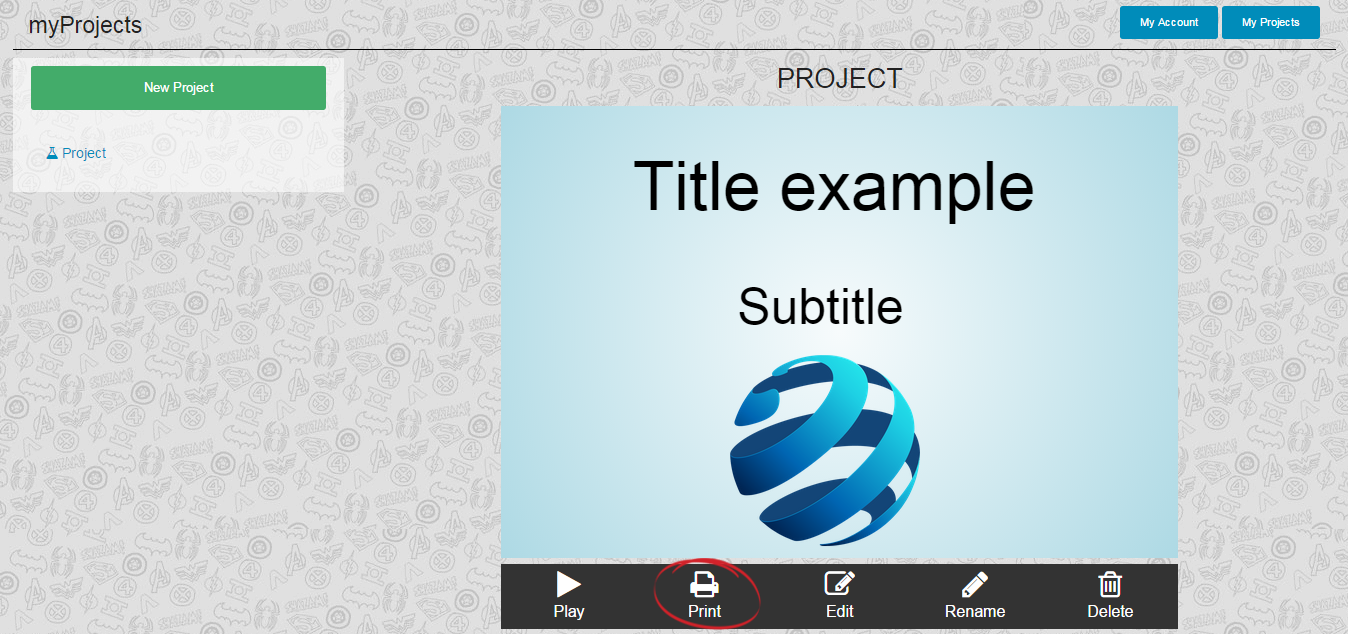
\includegraphics[scale=0.40] {img/stampa_pro.png}
	\caption{Stampa ed esportazione di un progetto} 
\end{figure}

\noindent Selezionando dal menù la voce \textbf{Print} si aprirà una nuova scheda dove verrà visualizzata l'intera presentazione come un'unica pagina web. Le slide\ped{G} verranno impaginate verticalmente una sotto l'altra nell'ordine in cui vengono visualizzate nella presentazione.

\begin{figure}[H] 
	\centering 
	
\includegraphics[scale=0.40] {img/print.png}
	\caption{Stampa ed esportazione di un progetto - Presentazione come un'unica pagina} 
\end{figure}

\subsection{Stampa di una presentazione}
\noindent Nel caso in cui si voglia stampare la presentazione è sufficiente utilizzare la funzione stampa presente nel browser\ped{G} che si sta utilizzando. Per ogni chiarimento in merito è consigliata la consultazione del manuale d'utilizzo del proprio browser\ped{G}. 

\subsection{Esportazione di una presentazione}
Nel caso in cui si voglia esportare la presentazione in formato PDF\ped{G} si dovrà utilizzare la funzionalità di stampa presente in Google Chrome\ped{G} e successivamente sfruttare la stampa su file. Di seguito verrà indicata la procedura da seguire, per questa guida è stata usata la versione 42 di Google Chrome\ped{G}. Una volta selezionata la funzionalità di stampa, apparirà la seguente schermata:

\begin{figure}[H] 
	\centering 
	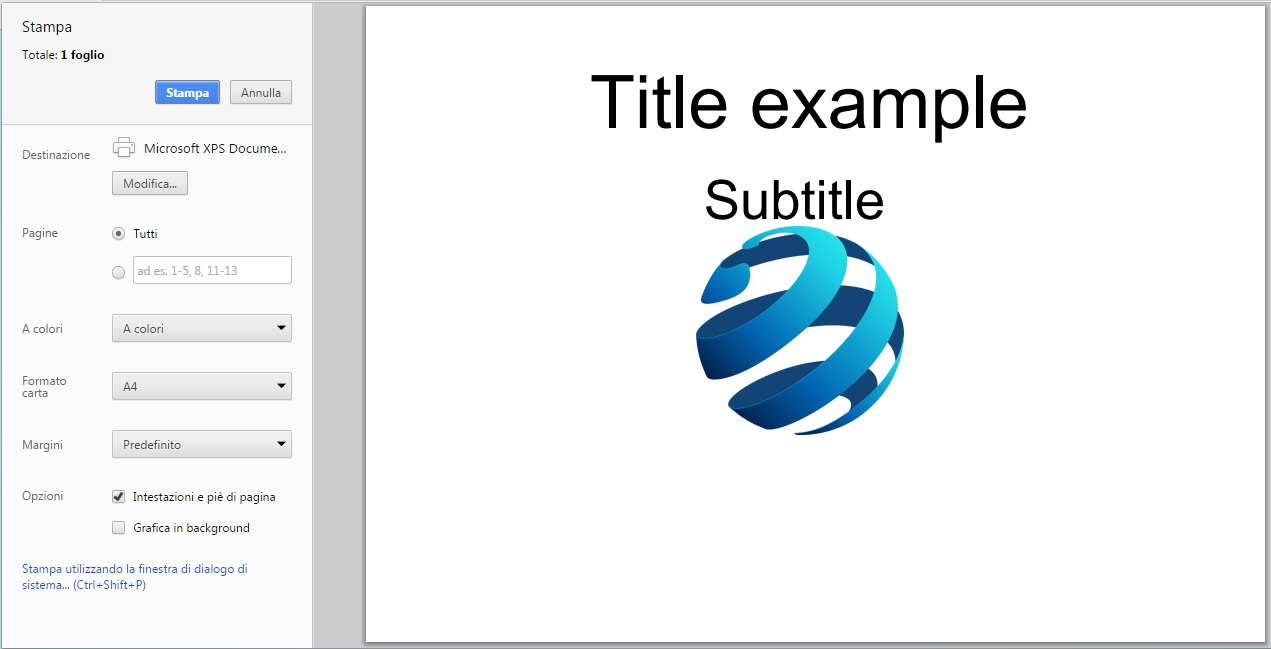
\includegraphics[scale=0.40] {img/print_google.png}
	\caption{Stampa ed esportazione di un progetto - Esportazione in formato PDF con Google Chrome} 
\end{figure}

\noindent Nel menù laterale di sinistra, a fianco alla voce \textit{Destinazione} selezionare il pulsante \textbf{Modifica...} e successivamente selezionare la voce \textit{Salva come PDF\ped{G}} (vedi figura sotto): 

\begin{figure}[H] 
	\centering 
	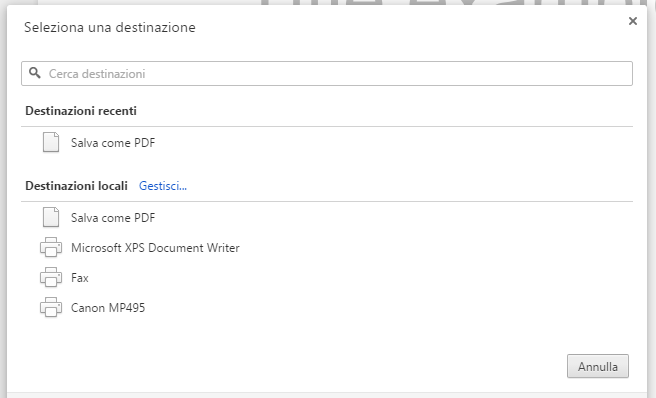
\includegraphics[scale=0.40] {img/salvacome.png}
	\caption{Stampa ed esportazione di un progetto - Settaggio stampa PDF con Google Chrome} 
\end{figure}

\noindent Una volta seguiti questi passi sarà sufficiente premere il pulsante di colore blu \textbf{Salva} e scegliere la destinazione di salvataggio della presentazione. 